\section{引言与问题重述}
\subsection{问题背景}

我国南方山区地形起伏剧烈、沟谷深切，洪涝灾害发生后常出现道路塌方中断、电力与通信基站损毁的复合灾情。此时地面车辆难以在黄金救援期内抵达受灾村镇，“最后一公里”的物资投送与应急通信保障成为救援成败的关键。无人机具有起降场地要求低、受地形阻隔影响小、可快速部署的优点，已在应急物资投送、灾情侦察与临时通信中继等场景中得到应用\cite{yang2026dronehumanitarian,zhang2021truckdrone,wang2014reliefrouting}。

然而山区场景下的无人机运用面临三重耦合困难：\textbf{其一}，地形起伏直接决定航段必须爬升的高度，进而通过爬升能耗与载荷—航程关系影响单架次能力；\textbf{其二}，山体遮挡会造成视距链路中断，而应急通信要求运输无人机在爬升、巡航、下降与投送\textbf{全程}保持通信，必须引入中继无人机并合理选址；\textbf{其三}，机队规模、机型异构程度、共享电池数量与充电周转时间共同构成资源约束，使“能否按时送达”不再只是路径优化问题，而是\textbf{机队并行能力与调度规则共同决定}的资源—调度耦合问题。

本文以某山区乡镇的洪涝灾害救援为背景。临时调度中心 O01 同时是固定通信网关 G01 的所在地，下辖 15 个服务区，共需投送 80 个不可拆分的货箱，其中 30 个为“首批保障”货箱并附带更严格的截止时间。可用装备为 3 种型号共 8 架运输无人机、2 架中继无人机，以及按机型独立配置的共享电池与中继能源组件。区域 30\,m 数字高程模型（DEM）与通信链路预算参数由附件给出。

\subsection{问题重述}

\noindent \textbf{问题 1（单点往返运输能力与货箱组批）}：针对 3 种运输机型与 15 个服务区，确定每种机型在各服务区的\textbf{最大安全载荷}；在此基础上为每个服务区设计货箱组批方案，在满足载质量、装载体积与返航安全能量余量的前提下，综合往返架次数、总运输能耗与累计作业时间说明目标间的权衡关系，并分析返航安全余量 $\rho_{g}$ 变化对结果的影响。

\noindent \textbf{问题 2（异构无人机多点多架次运输调度）}：允许单个架次访问一个或多个服务区，联合确定货箱组批、服务区访问顺序、运输机型、具体执行的实体无人机、共享电池分配与各架次开始时刻，在货物不可拆、载质量与体积、返航安全余量、无人机与电池数量以及充电周转等约束下，优化配送及时性、全部任务完成时间、运输能耗与架次数，并检验方案的资源可行性。

\noindent \textbf{问题 3（通信约束下的运输与中继联合调度）}：在问题 2 的基础上引入\textbf{连续通信约束}——运输无人机在爬升、巡航、下降及物资投送阶段均应保持通信。需联合确定中继无人机的悬停位置（含平面位置与飞行海拔）、服务时段与能源组件分配，在悬停离地高度上限、返航电量、不允许多跳转发等约束下，给出运输与中继的联合调度方案，并说明货箱交付、资源使用与通信保障三类情况。

\noindent \textbf{问题 4（救援任务分区与资源配置优化）}：以问题 3 的联合调度方案为基础，将 15 个服务区划分为 \textbf{2 组}与 \textbf{3 组}两种任务分区方案，\textbf{保持问题 3 已确定的货箱组批、访问顺序、任务安排与通信保障关系不变}，且\textbf{同一运输架次涉及的服务区必须划入同一任务组}；各任务组仅承担本组任务、资源不得跨组调配。需核算每组独立执行所需的运输无人机、共享电池、中继无人机与中继能源组件数量，并从配置规模、资源冗余、组间工作量均衡与资源缺口四方面比较两种分区。

\subsection{总体技术路线}

围绕上述四个层层递进的问题，本文确立“\textbf{统一口径 $\rightarrow$ 逐问建模 $\rightarrow$ 独立校验}”的技术路线：先构建四问共用的公共物理与通信模型，杜绝口径分叉；再按问题一到问题四依次求解，后一问严格继承前一问的方案；最后用独立复算对全部结果做交叉验证。全文技术路线如图~\ref{fig:roadmap} 所示。

\begin{figure}[htbp]
	\centering
	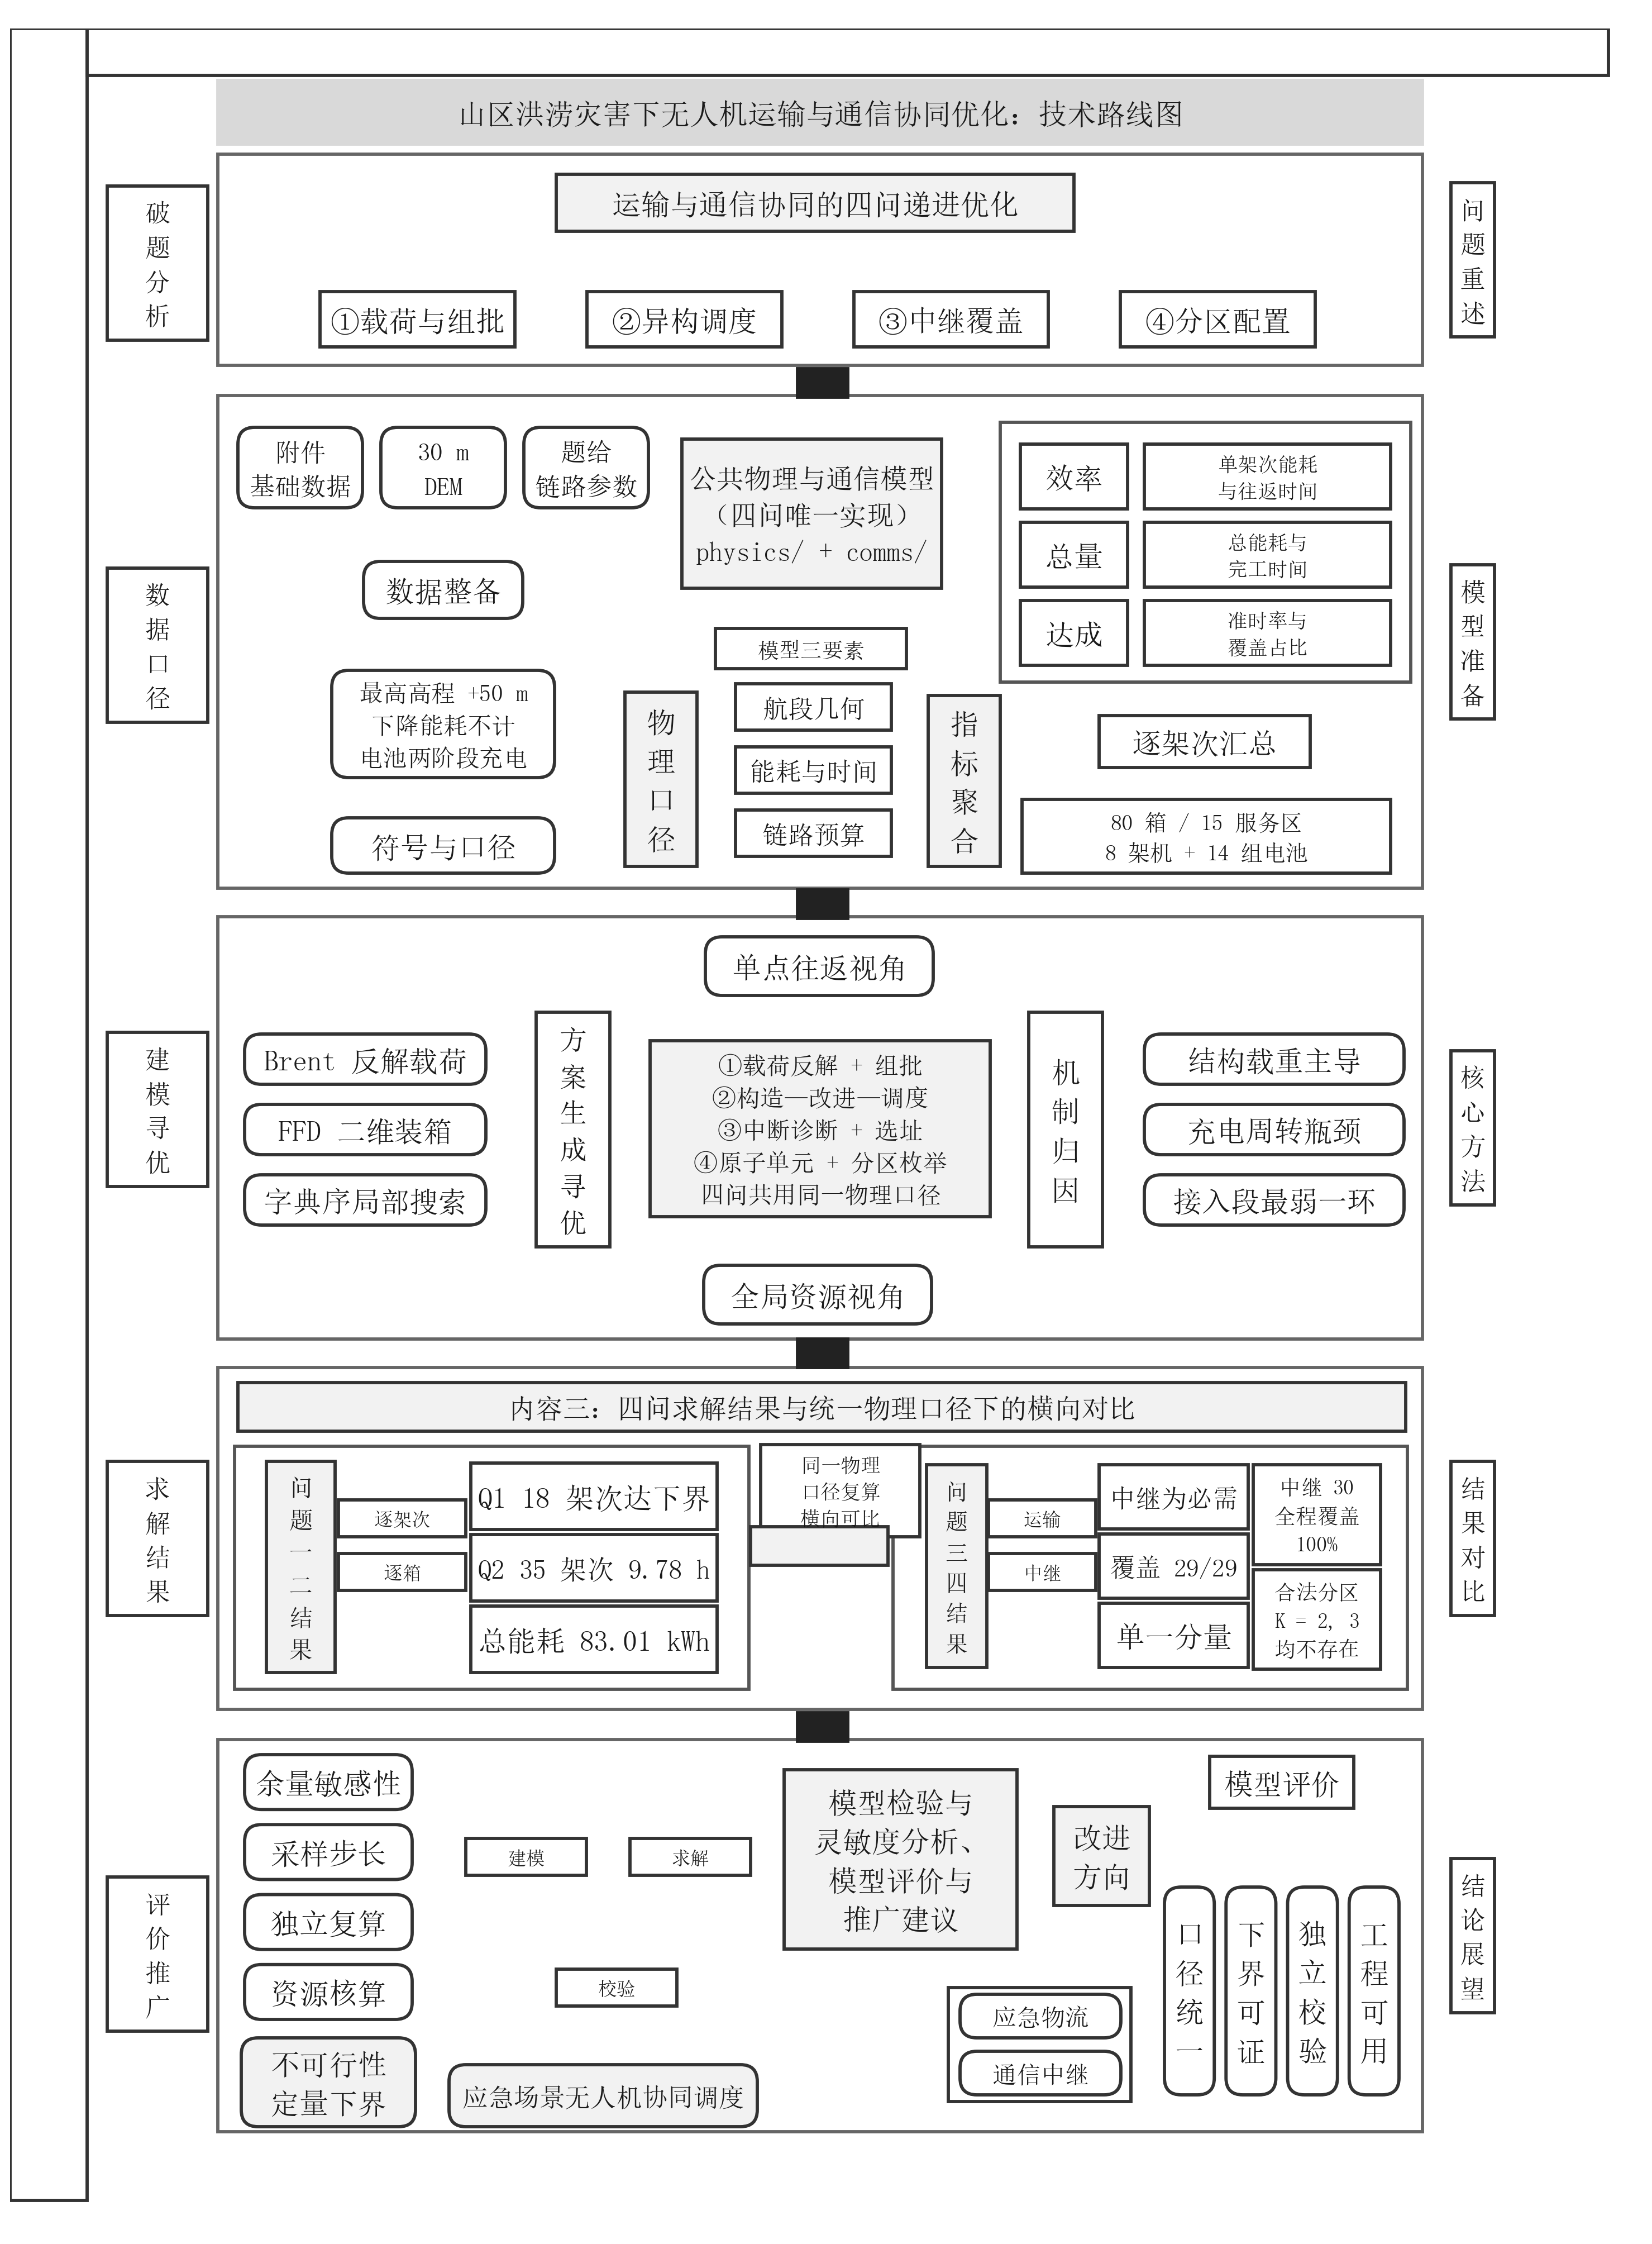
\includegraphics[width=0.70\textwidth]{figures/fig01_roadmap.png}
	\caption{全文技术路线图}
	\label{fig:roadmap}
\end{figure}

如图~\ref{fig:roadmap} 所示，全文沿“破题分析—数据口径—建模寻优—求解结果—评价推广”五个层次递进展开。第一层把总命题“运输与通信协同的四问递进优化”拆分为载荷与组批、异构调度、中继覆盖、分区配置四个并列子问题；第二层明确数据来源（附件基础数据、30\,m DEM、题给链路参数）与三条核心口径（航段取最高高程 $+50$\,m、下降能耗不单独计、电池两阶段充电）；第三层给出四问各自的核心方法，并归因出三条机制性结论（结构载重主导、\textbf{异构机队必须混编以取得并行度}、中继接入段最弱）；第四层在统一物理口径下横向对比四问结果，其中“通信覆盖 100\%（24/24）”与“合法组数受原子单元拓扑支配（原子单元 5 个，$K=2$、$K=3$ 均可零架次改动实现）”是最具区分度的两个结论；第五层给出模型检验、灵敏度分析与推广方向。
